\section{Length Of A Vector}
\label{sec:length-of-a-vector}

In this section we generalise the `intuitive' understanding of a vector's length
readers might have acquired in dimensions one and two.

Starting low, in dimension one, a vector with one entry is basically just a real
number. It represents a shift on an infinite line to the right or left starting
at $0$. In this case, its length is clearly just the \emph{absolute value} of
its single entry. Nonetheless, it's appropriate to remind ourselves how absolute
value is actually defined. For a number $x \in \R$, we define its \emph{absolute
value} to be
\[
 |x| \coloneqq \sqrt{x^2}.
\]
This means that the length of a vector $\mathbf{v} = (v_1)$ with a single entry
$v_1 \in \R$ comes out to be exactly $\sqrt{v_1^2}$. We shall denote the length
of a vector $\mathbf{v}$ as $\|\mathbf{v}\|$, also called its \emph{norm}.

In dimension two, things complicate a tad. A vector now comprises two real
entries, the horizontal shift and the vertical one. Thankfully, the well-known
and loved \emph{Pythagorean Theorem} comes to the rescue. The important idea
here is to literally split a vector into its horizontal and vertical part. We
mean it like this: given a vector
\[
 \mathbf{v} =
 \begin{pmatrix}
  v_1\\
  v_2
 \end{pmatrix},
\]
we construct vectors $\mathbf{v}_x$ and $\mathbf{v}_y$ like this:
\[
 \mathbf{v}_x \coloneqq
 \begin{pmatrix}
  v_1\\
  0
 \end{pmatrix}, \quad 
 \mathbf{v}_y \coloneqq 
 \begin{pmatrix}
  0\\
  v_2
 \end{pmatrix}.
\]
Now, we have $\mathbf{v} = \mathbf{v}_x + \mathbf{v}_y$ and we know that
$\|\mathbf{v}_x\| = |v_1|$ and $\|\mathbf{v}_y\| = |v_2|$. Since $\mathbf{v}_x$
and $\mathbf{v}_y$ are the legs of a right triangle with hypotenuse
$\mathbf{v}$ (see \myref{figure}{fig:vector-pythagoras}), we arrive at the
equation
\[
 \|\mathbf{v}\|^2 = \|\mathbf{v}_x\|^2 + \|\mathbf{v}_y\|^2,
\]
from which it follows that
\[
 \|\mathbf{v}\| = \sqrt{\|\mathbf{v}_x\|^2 + \|\mathbf{v}_y\|^2} = \sqrt{|v_1|^2
 + |v_2|^2} = \sqrt{v_1^2 + v_2^2},
\]
where the last equality holds because $v_1^2$ and $v_2^2$ are positive
regardless of whether $v_1$ and $v_2$ are.
  
\begin{figure}[ht]
 \centering
 \begin{tikzpicture}
  \tkzInit[xmin=-2,xmax=3,ymin=-1,ymax=3]
  \tkzDrawX[arrows={-Latex[width=4pt,length=6pt]},dashed,label=]
  \tkzDrawY[arrows={-Latex[width=4pt,length=6pt]},dashed,label=]
  \tkzDefPoints{2/3/a,2/0/a1,0/3/a2,0/0/O}
  \tkzDrawSegment[-Latex,thick,BrickRed](O,a1)
  \tkzDrawSegment[-Latex,thick,RoyalBlue](a1,a)
  \tkzDrawSegment[-Latex,thick,ForestGreen](O,a)
  \tkzLabelSegment[BrickRed,below](O,a1){$\mathbf{v}_x$}
  \tkzLabelSegment[RoyalBlue,right](a1,a){$\mathbf{v}_y$}
  \tkzLabelSegment[ForestGreen,above=1mm](O,a){$\mathbf{v}$}
 \end{tikzpicture}
 \caption{Computing the length of $\clg{\mathbf{v}} = \clr{\mathbf{v}_x} +
 \clb{\mathbf{v}_y}$ using the Pythagorean Theorem.}
 \label{fig:vector-pythagoras}
\end{figure}

An analogous approach will also work in dimension three. Here we instead break a
vector into three components. That is, given a vector
\[
 \mathbf{v} = 
 \begin{pmatrix}
  v_1\\
  v_2\\
  v_3
 \end{pmatrix}
\]
we break it up into
\[
 \mathbf{v} =
 \begin{pmatrix}
  v_1\\
  v_2\\
  v_3
 \end{pmatrix}
 = 
 \begin{pmatrix}
  v_1\\
  0\\
  0
 \end{pmatrix}
 + 
 \begin{pmatrix}
  0\\
  v_2\\
  0
 \end{pmatrix}
 + 
 \begin{pmatrix}
  0\\
  0\\
  v_3
 \end{pmatrix}
 = \mathbf{v}_x + \mathbf{v}_y + \mathbf{v}_z.
\]
Just as before, we know that $\|\mathbf{v}_x\| = |v_1|$, $\|\mathbf{v}_y\| =
|v_2|$ and $\|\mathbf{v}_z\| = |v_3|$. The vector
\[
 \mathbf{v}_{xy} = \mathbf{v}_x + \mathbf{v}_y
\]
is the hypotenuse of the right triangle with legs $\mathbf{v}_x$ and
$\mathbf{v}_y$. This means that
\[
 \|\mathbf{v}_{xy}\| = \sqrt{\|\mathbf{v}_x\|^2 + \|\mathbf{v}_y\|^2} =
 \sqrt{v_1^2 + v_2^2}.
\]
Similarly, the vector $\mathbf{v}$ itself is a hypotenuse of the right triangle
formed by vectors $\mathbf{v}_{xy}$ and $\mathbf{v}_z$. It follows that
\[
 \|\mathbf{v}\| = \sqrt{\|\mathbf{v}_{xy}\|^2 + \|\mathbf{v}_z\|^2} =
 \sqrt{v_1^2 + v_2^2 + v_3^2}.
\]

\begin{figure}[ht]
 \centering
 \begin{tikzpicture}
  \tkzDefPoints{2/0/x,3/1/y,3/3/z,0/0/O}
  \tkzDrawSegment[-Latex,thick,BrickRed](O,x)
  \tkzDrawSegment[-Latex,thick,RoyalBlue](x,y)
  \tkzDrawSegment[-Latex,thick,ForestGreen](y,z)
  \tkzLabelSegment[BrickRed,below](O,x){$\mathbf{v}_x$}
  \tkzLabelSegment[RoyalBlue,below right](x,y){$\mathbf{v}_y$}
  \tkzLabelSegment[ForestGreen,right](y,z){$\mathbf{v}_z$}

  \tkzDrawSegment[-Latex,dashed](O,y)
  \tkzLabelSegment[above right=2mm and 0](O,y){$\mathbf{v}_{xy}$}
  \tkzDrawSegment[-Latex,Fuchsia,thick](O,z)
  \tkzLabelSegment[Fuchsia,above left](O,z){$\mathbf{v}$}
  \tkzMarkRightAngle[size=4mm,german](y,x,O)
  \tkzMarkRightAngle[size=4mm,german](z,y,O)
 \end{tikzpicture}
 \caption{Computing the length of the vector $\clg{\mathbf{v}} =
  \clr{\mathbf{v}_x} + \clb{\mathbf{v}_y} + \clm{\mathbf{v}_z}$ using the
  Pythagorean Theorem twice.}
 \label{fig:vector-pythagoras-3d}
\end{figure}

Hopefully kind readers have begun to see the pattern. We can split a vector
\[
 \mathbf{v} =
 \begin{pmatrix}
  v_1\\
  v_2\\
  \vdots\\
  v_n
 \end{pmatrix}
\]
into `basically one-dimensional' vectors
\[
 \mathbf{v}_{x_1} =
 \begin{pmatrix}
  v_1\\
  0\\
  0\\
  \vdots\\
  0
 \end{pmatrix},
 \mathbf{v}_{x_2} = 
 \begin{pmatrix}
  0\\
  v_2\\
  0\\
  \vdots\\
  0
 \end{pmatrix},\ldots,
 \mathbf{v}_{x_n} = 
 \begin{pmatrix}
  0\\
  0\\
  0\\
  \vdots\\
  v_n
 \end{pmatrix}.
\]
and calculate its length as the length of the body diagonal of the
$n$-dimensional cuboid with side lengths $\|\mathbf{v}_{x_1}\|,
\|\mathbf{v}_{x_2}\|, \ldots, \|\mathbf{v}_{x_n}\|$. Let us first prove that
said body diagonal indeed has the length we expect.

\begin{lemma}{Body diagonal of a cuboid}{body-diagonal-of-a-cuboid}
 The length of the body diagonal of an $n$-dimensional cuboid with side lengths
 $a_1,a_2,\ldots,a_n$ is exactly $\sqrt{a_1^2 + a_2^2 + \ldots + a_n^2}$.
\end{lemma}
\begin{lemproof}
 We prove the lemma by induction on the dimension of the cuboid.

 A cuboid of dimension one has only one side of length $a_1$ and thus its body
 diagonal consists of just this single side and is therefore long exactly $a_1 =
 |a_1| = \sqrt{a_1^2}$. Thus, the base case is handled.

 Now, consider an $(n-1)$-dimensional cuboid $C_{n-1}$ with side lengths
 $a_1,\ldots,a_{n-1}$ and assume its body diagonal has length $\sqrt{a_1^2 +
 a_2^2 + \ldots + a_{n-1}^2}$. Adding a dimension to $C_{n-1}$ means regarding
 $C_{n-1}$ as the base of the $n$-dimensional cuboid $C_n$ with side lengths
 $a_1,a_2,\ldots,a_n$ (imagine the square being a base for the cube). By
 definition, this added side is perpendicular to the entirety of $C_{n-1}$. In
 particular, the body diagonal of $C_{n-1}$ is perpendicular to the newly added
 side of length $a_n$. This means that the body diagonal of $C_n$ is the
 hypotenuse in the right triangle formed by the body diagonal of $C_{n-1}$ and
 the side of length $a_n$ of $C_n$. The Pythagorean theorem now reads that the
 length of the body diagonal of $C_n$ is exactly
 \[
  \sqrt{\left( \sqrt{a_1^2 + a_2^2 + \ldots + a_{n-1}^2} \right)^2 + a_n^2} =
  \sqrt{a_1^2 + a_2^2 + \ldots + a_{n-1}^2 + a_n^2}
 \]
 and the lemma is hence proven.
\end{lemproof}

The previous lemma justifies the definition of the length of a vector which we
promptly proceed to utter.

\begin{definition}{Length of a vector}{length-of-a-vector}
 The length of a vector $\mathbf{v} \in \R^{n}$ with entries $v_1,\ldots,v_n$ is
 defined as
 \[
  \|\mathbf{v}\| \coloneqq \sqrt{v_1^2 + v_2^2 + \ldots + v_n^2}.
 \]
\end{definition}

